\documentclass[conference]{IEEEtran}
\usepackage{graphicx}
\usepackage{url}
\usepackage{pbox}
\usepackage{xcolor}
%\usepackage[colorlinks]{hyperref}
%\hypersetup{linkcolor=blue, citecolor=blue, urlcolor=blue}

\DeclareGraphicsExtensions{.pdf,.png,.jpg}
\graphicspath{{./ImportedFigures/}}

\ifCLASSINFOpdf
\else
\fi
\hyphenation{op-tical net-works semi-conduc-tor}

\newif\ifdraft
\drafttrue
\ifdraft
\usepackage{xcolor}
\usepackage{array}
\usepackage{makecell}
\renewcommand\cellalign{cl}
\definecolor{ocolor}{rgb}{1,0,0.4}
\newcommand{\aanote}[1]{ {\textcolor{red} { ***amy: #1 }}}
\newcommand{\alnote}[1]{ {\textcolor{blue} { ***andre: #1 }}}
\newcommand{\ednote}[1]{ {\textcolor{brown} { ***eddie: #1 }}}
\newcommand{\kknote}[1]{ {\textcolor{green} { ***ken: #1 }}}
\newcommand{\dungnote}[1]{ {\textcolor{orange} { ***dung: #1 }}}
\else
\newcommand{\aanote}[1]{}
\newcommand{\alnote}[1]{}
\newcommand{\ednote}[1]{}
\newcommand{\kknote}[1]{}
\newcommand{\dungnote}[1]{}
\fi

\begin{document}

\title{Deep Stream: Edge-to-Cloud Stream Processing for Deep Learning Computer Vision Applications in  Automotive Manufacturing}
% * <dungx.ngt@gmail.com> 2017-10-02T03:34:15.504Z:
%
% ^.


\maketitle

% These two lines add back the page numbers; we may need to remove
% before submitting
\thispagestyle{plain}
\pagestyle{plain}



\begin{abstract}
In this paper, we investigate the trade-off between resource/cost consumption with running time and accuracy of different object detector models based on deep neural networks.
\end{abstract}


\IEEEpeerreviewmaketitle


%%%%%%%%%%%%%%%%%%%%%%%%%%%%%%%%%%%%%%%%%%%%%%%%%%%%%%
\section{Introduction and Motivating Application}
%%%%%%%%%%%%%%%%%%%%%%%%%%%%%%%%%%%%%%%%%%%%%%%%%%%%%%

We aim to compare different families of object detectors in different devices: from state-of-the-art multiple GPUs workstations to resource-limited devices such as mini computers (Raspberry Pi, NIVDIA ...) and mobile devices (iPhone) or deep learning-specialized devices (Amazon DeepLens).

\alnote{Motivate streaming}

The difficulties of this project come from the differences of deep learning framework environments on different devices with different levels of optimization and efficiency, the wide varieties of object detectors, in both meta-architectures and feature extractors. 

For our applications, we only consider the test-time performance, which concerns about inference time, deployment time, memory footprint and hardware utilization in test-time only.

We illustrate a big picture of deep network object detectors for many different devices and purposes. Very light-weight devices such as Raspberry Pi require a small network and efficient run time environment to produce minimal memory footprint. Other devices requires real-time processing time to provide smooth user experience, particularly on smartphones. Different applications and devices have their own unique requirements and characteristics. 
%%%%%%%%%%%%%%%%%%%%%%%%%%%%%%%%%%%%%%%%%%%%%%%%%%%%%%
\section{Architecture Backgrounds}
%%%%%%%%%%%%%%%%%%%%%%%%%%%%%%%%%%%%%%%%%%%%%%%%%%%%%%
There are multiple degrees of freedom in an object detector model:

\begin{itemize}
    \item Meta-Architecture: SSD, DeepMultiBox, R-FCN, Faster R-CNN, YOLO, ...
    \item Feature Extractor: VGG (multiple versions), Resnet (m), Inception (m), Inception Resnet, MobileNet. At least 6 are reported in~\cite{huang2017speed}. Feature Extractors are pre-trained on ImageNet-CLS (Image Classification task) first, and then are used to initialize the complete networks. 
    \item Feature Layers: Select which layer(s) of the feature extractor to be used in Meta-Architecture. Several papers select top (deepest) convolutional layer, but other papers encourage to aggregate multiple layers, even fully-connected layers.
    \item Box Proposals: Different original paper reports different number of proposals (10 .. 300 for an image of ~300x300 pixels)
    \item Trained Image size: 300 .. 600: R-FCN and Faster R-CNN are fixed at shorter edge. SSD is fixed at both edges.
    \item Stride (in feature extractor): reports show that stride is an important factor in the trade-off between performance (in mAP) and running time.
\end{itemize}

Original papers usually just report 1 single combination of these options, with several variants.

\dungnote{A strong argument against using original models but not combinations is the original models are optimized to get highest accuracy but not taking into account other trade-off such as memory or inference time. Several original models use different complex data augmentation methods. Another issue is original papers report results on different combinations of training sets (2007/2012 PASCAL VOC eval, 2007+2012 PASCAL VOC eval + test, etc}

\dungnote{A good thing is the paper at~\cite{huang2017speed} already produced a pipeline to re-train all the setup combinations. Therefore we only need to add/implement parts of new combinations. Source code can be found on Github. Training/Evaluation can be done only once in powerful workstations. We only need to record running time and resource utilization at edge devices.}

\subsection{Meta-Architectures}

\alnote{good practical overview: \url{https://github.com/datadynamo/aiconf_ny_2018_pytorch_cv_tutorial/blob/master/AIConf_April2018_PyTorch_Computer_Vision_Part2.pdf}}

\alnote{Yolo v3?}
In general, SSD and YOLOv2 are used for fast, low-latency jobs while Faster R-CNN is often used for higher accuracy.

\subsubsection{SSD}
This one is the fastest meta-architecture. SSD is more flexible~\alnote{what does flexible mean?} than YOLO because it uses prior boxes at different aspect ratio at different scale of feature map.~\cite{liu2016ssd}

The original models are trained on PASCAL VOC (2007 and 2012 versions) and 2014 ILRSVRC datasets.

\subsubsection{Faster R-CNN}
Faster R-CNN, which yields high accuracy object detection results, is a model that derived from R-CNN~\cite{girshick2015fast}.

R-CNN is originally pre-trained on PASCAL VOC 2007 and fine-tuned on PASCAL VOC 2012 datasets. 

\subsubsection{DeepMultiBox}

\subsubsection{YOLO and YOLO v2}
YOLO also uses single neural network without proposal generation process, combined with a customized feature extractor derived from GoogLeNet to predict classes and shapes of objects.

\subsubsection{R-FCN}
R-FCN improves Faster R-CNN by delaying the cropping process to deeper layers of the net.

\subsubsection{SPPnet}
Improved version of R-CNN. This meta-architecture is out performed by Fast R-CNN and Faster R-CNN.

\subsection{Feature Extractors}

\subsubsection{MobileNet}
MobileNet is an efficient deep net that is able to produce relatively light-weight networks but still have reasonable performance. ~\cite{howard2017mobilenets}

\subsubsection{VGG (Outdated)}

\subsubsection{Inception V3}

\subsubsection{Resnet}

\subsubsection{SqueezeNet}
This is a very light-weighted deep learning network~\cite{shen2018cs}

\subsubsection{XNOR Net}
This is a variant of binary weights network, operations in convolution layers are approximated by bit-wise operations (XNOR)~\cite{rastegari2016xnor}.
%%%%%%%%%%%%%%%%%%%%%%%%%%%%%%%%%%%%%%%%%%%%%%%%%%%%%%
\section{Model Combinations}
%%%%%%%%%%%%%%%%%%%%%%%%%%%%%%%%%%%%%%%%%%%%%%%%%%%%%%

\subsection{Original Models}

\begin{figure*}[htpb]
	  \centering
	  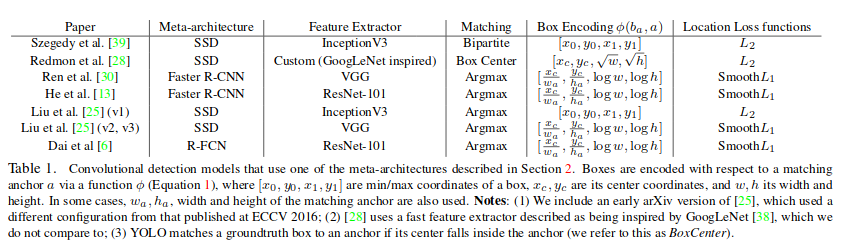
\includegraphics[width=1\textwidth]{original_models_1}
	  \caption{Original combinations reported in other researches.}
	  \label{fig:original_combinations}
\end{figure*}

%%%%%%%%%%%%%%%%%%%%%%%%%%%%%%%%%%%%%%%%%%%%%%%%%%%%%%
\section{Devices and Environment Setup}
%%%%%%%%%%%%%%%%%%%%%%%%%%%%%%%%%%%%%%%%%%%%%%%%%%%%%%

\subsection{Devices}
In this section, we present the comparison between features and cost/power consumption of tested devices


\subsection{Deep Learning Frameworks}
DeepX Toolkit is a framework used in resource efficiency deep learning optimization.

%%%%%%%%%%%%%%%%%%%%%%%%%%%%%%%%%%%%%%%%%%%%%%%%%%%%%%
\section{Performance Metrics}
%%%%%%%%%%%%%%%%%%%%%%%%%%%%%%%%%%%%%%%%%%%%%%%%%%%%%%

\subsection{Accuracy on ImageNet}
The common metric to measure accuracy in object detection is mAP.

The performance on ImageNet of several models in this paper are reported in original papers and other  researches~\cite{huang2017speed}.


\subsection{Deep Learning Performance}

MLPerf, \url{https://mlperf.org/}

%%%%%%%%%%%%%%%%%%%%%%%%%%%%%%%%%%%%%%%%%%%%%%%%%%%%%%
\section{Experimental Results}
%%%%%%%%%%%%%%%%%%%%%%%%%%%%%%%%%%%%%%%%%%%%%%%%%%%%%%

%%%%%%%%%%%%%%%%%%%%%%%%%%%%%%%%%%%%%%%%%%%%%%%%%%%%%%
\section{Analysis}
%%%%%%%%%%%%%%%%%%%%%%%%%%%%%%%%%%%%%%%%%%%%%%%%%%%%%%
Discussion about trade-off in streaming environment is analyzed and discussed in this section.

%%%%%%%%%%%%%%%%%%%%%%%%%%%%%%%%%%%%%%%%%%%%%%%%%%%%%%
\section{Related Works}
%%%%%%%%%%%%%%%%%%%%%%%%%%%%%%%%%%%%%%%%%%%%%%%%%%%%%%
~\cite{huang2017speed}~do a similar research, but their experiments are limited to powerful workstations, in which the implementations of the models are developed using Tensorflow framework. The accuracy of this paper's models are evaluated on COCO for object detection.

%%%%%%%%%%%%%%%%%%%%%%%%%%%%%%%%%%%%%%%%%%%%%%%%%%%%%%
\section{Conclusion}
%%%%%%%%%%%%%%%%%%%%%%%%%%%%%%%%%%%%%%%%%%%%%%%%%%%%%%

\bibliographystyle{unsrt}
%\bibliographystyle{abbrv}
%\setstretch{1}
%\setlength\bibitemsep{0pt}
\bibliography{deeplearning}




% that's all folks
\end{document}

